\documentclass[12pt, titlepage]{article}

\usepackage{graphicx} % Allows for images
\usepackage{wrapfig} % Allows for text wrapping around images
\usepackage{hyperref} % Allows for hyperlinks
\usepackage{siunitx} % Allows for SI units
\usepackage{amsmath} % Allows for math
\usepackage{enumerate} % Allows for custom enumerations
\usepackage{xcolor} % Allows for custom colors
\usepackage{tikz, tcolorbox} % Allows for custom boxes
\usepackage{microtype} % Allows for better text alignment
\usepackage{listings} % Allows for code listings
\usepackage{booktabs} % Allows for better tables
\usepackage{float} % Allows for better figure placement
\usepackage{geometry} % Allows for custom page geometry
\usepackage{fancyhdr} % Allows for custom headers and footers
\usepackage{caption} % Allows for custom captions

\fancypagestyle{myarticlestyle}{
    \fancyhf{} % Clear header and footer
    \fancyhead[L]{\leftmark} % Section name on the left
    \fancyhead[R]{\thepage} % Page number on the right
}
\fancypagestyle{tocstyle}{
    \fancyhf{} % Clear header and footer
    \fancyhead[L]{CONTENTS} % Section name on the left
    \fancyhead[R]{\thepage} % Page number on the right
}

\pagestyle{myarticlestyle}
\setlength{\headheight}{15pt}

\title{Dynamic Force Analysis}
\author{Omar Ebrahim 110076575\\Dr. Bill Altenhof\\ University of Windsor}

\begin{document}
\maketitle
\newpage
\tableofcontents
\listoffigures
\listoftables
\thispagestyle{tocstyle}
\newpage
\section{Introduction}
Mechanical systems involving the interaction of various components play a
crucial role in understanding and optimizing the performance of machines. In
this lab report, a dynamic force analysis will be conducted for an opposed
two-cylinder crank/connecting rod/slider arrangement. 
\subsection{Objectives}
The primary objective of this analysis is to delve into the kinematic and
kinetic aspects of the system. Through numerical and symbolic calculations, we
aim to determine key parameters, including angular velocities, angular
accelerations, transmitted forces, input torque for constant angular velocity,
and out-of-balance forces. These parameters will be crucial in comprehending
the system's behavior and optimizing its design.\\[10pt]
The investigation encompasses a time-dependent analysis covering two complete
revolutions of the crank, and the obtained results will be graphically
illustrated.
\subsection{Approach}
The analysis will be carried out utilizing computational
software, namely MATLAB, and analytical methods. The analytical equations
developed in class will be employed to conduct a comprehensive analysis of the
system, particularly in determining the out-of-balance forces. The MATLAB
software will be used to numerically solve the system's equations of motion.\\[10pt]
This dual approach, combining computational tools and analytical methods,
ensures a robust and comprehensive understanding of the mechanical system under
consideration.
\newpage
\subsection{Literature Review}
In the domain of dynamic force analysis for levitated planar actuators,
Rovers\footnote{Rovers, (2012)} makes a substantial contribution. Their paper
meticulously explores the dynamic forces and torques exerted within a moving
planar actuator, shedding light on crucial aspects of its behavior.\\[10pt]
The work by Korayem\footnote{Korayem, (2011)} stands out for its notable
significance in the dynamic analysis of tapping-mode Atomic Force Microscopy
(AFM). The paper focuses specifically on capillary force interactions,
enriching our understanding of the intricacies involved.\\[10pt]
Similarly, Williams\footnote{Williams, (1981)} contributes significantly to the
field with a study centered on the dynamic force analysis of planar mechanisms.
The insights provided in this work are valuable for comprehending the nuanced
behavior of such systems.\\[10pt]
Cheng-ge\footnote{Cheng-ge, (2010)} adds to the discourse with noteworthy
research on the dynamic force analysis of power capacitors within a frame
context. The detailed exploration carried out in this paper makes a substantial
contribution to the relevant body of knowledge.\\[10pt]
Lastly, the work by Schütte\footnote{Schütte, (2015)} holds considerable
importance, delving into the discussion of ConDroid, a tool designed for
targeted dynamic analysis of Android applications. This contribution extends
the scope of analysis beyond mechanical systems, showcasing the
interdisciplinary nature of dynamic force examination.\\[10pt]
Collectively, these papers form a robust foundation for the comprehensive analysis of the mechanical system under consideration.
\newpage
\section{Methodology}
The methodology section will outline the approach taken to conduct the analysis
and the tools utilized.
\subsection{Analytical Approach}
The analytical approach will be employed to determine the out-of-balance forces
and the input torque for constant angular velocity. The equations of motion
will be derived using the Newton-Euler method, and the out-of-balance forces
will be determined using the method of dynamically equivalent masses and 
force balancing.\\[10pt]
The Newton-Euler method is a powerful tool for deriving the equations of motion
for a mechanical system. It involves the application of Newton's second law of
motion and Euler's equations of motion. The method is particularly useful for
systems with multiple degrees of freedom.\\[10pt]
The method of dynamically equivalent masses and force balancing is a
straightforward approach for determining the out-of-balance forces. It involves
the application of the principle of virtual work, and it is particularly useful
for systems with multiple degrees of freedom.
\subsection{Computational Approach}
The computational approach will be utilized to determine the angular
velocities, angular accelerations, and transmitted forces. The equations of
motion will be solved numerically using MATLAB.\\[10pt]
The MATLAB software is a powerful tool for solving complex equations. It
provides a robust platform for numerical analysis, and it is particularly
useful for solving systems of equations.
\newpage
\section{Analysis}
Assumptions made in the analysis include treating each linkage as a slender
rod, neglecting the effects of gravity and friction, and confining all motion
to a common plane. It is imperative to document and articulate any additional
assumptions deemed necessary for the analysis.\\[10pt]
The Required To Find (RTF) statements are as follows:
\begin{enumerate}
    \item Determine the angular velocities and angular accelerations of the
      crank, connecting rod, and slider.
    \item Determine the transmitted forces in the connecting rod and slider.
    \item Determine the input torque for constant angular velocity.
    \item Determine the out-of-balance forces.
\end{enumerate}
\subsection{Equations of Motion for Point A}
A diagram of the system is shown in Figure \ref{fig:system}. The diagram
shows the crank as well as point A rotating at $\omega$ radians per second
with angles $\theta$ and $\phi$ respectively.
\begin{figure}[H]
    \centering
    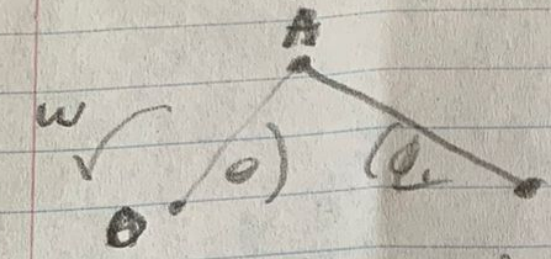
\includegraphics[width=0.8\textwidth]{./Images/f1.png}
    \caption{System Diagram}
    \label{fig:system}
\end{figure}
First, we will derive the equation of velocity for point A. The equation of
velocity for point A is given by:
\begin{equation}
    \label{eq:vel}
    \vec{v}_A = \omega \times \vec{r}_A \angle R\cos\theta + R\sin\theta
\end{equation}
Finding the x and y components of the equation of velocity for point A yields:
\begin{equation}
    \label{eq:velxy}
    \begin{split}
        v_{Ax} &= -R\omega\sin\theta\\
        v_{Ay} &= R\omega\cos\theta
    \end{split}
\end{equation}
Next, we will derive the equation of acceleration for point A. The equation of
acceleration for point A is given by:
\begin{equation}
    \label{eq:acc}
    \vec{a}_A = \omega \times (\omega \times \vec{r}_A) \angle
    R\cos\theta\omega^2, R\sin\theta\omega^2
\end{equation}
Finding the x and y components of the equation of acceleration for point A
yields:
\begin{equation}
    \label{eq:accxy}
    \begin{split}
        a_{Ax} &= -R\omega^2\cos\theta\\
        a_{Ay} &= -R\omega^2\sin\theta
    \end{split}
\end{equation}
\subsection{Equations of Motion for Point B}
\newpage
\section{Discussion}
\newpage
\section{Conclusions}
\newpage
\section{References}
\begin{enumerate}
    \item \label{item:cheng2010} Cheng-ge, H. (2010). Discussion on Frame
      Dynamic Force Analysis of Power Capacitor. Power Capacitor \& Reactive
      Power Compensation.

    \item \label{item:korayem2011} Korayem, M., Kavousi, A. \& Ebrahimi, N.
    (2011). Dynamic analysis of tapping-mode AFM considering capillary force
    interactions. Scientia Iranica.

    \item \label{item:rovers2012} Rovers, J., Jansen, J., Compter, J. \&
    Lomonova, E. (2012). Analysis Method of the Dynamic Force and Torque
    Distribution in the Magnet Array of a Commutated Magnetically Levitated
    Planar Actuator. IEEE transactions on industrial electronics (1982. Print).

    \item \label{item:shutte2015} Schütte, J., Fedler, R. \& Titze, D. (2015).
    ConDroid: Targeted Dynamic Analysis of Android Applications. 2015 IEEE 29th
    International Conference on Advanced Information Networking and
    Applications.

    \item \label{item:williams1981} Williams, R. \& Rupprecht, S. (1981). Dynamic
    force analysis of planar mechanisms. Mechanism and Machine Theory.
\end{enumerate}
\end{document}
